\RequirePackage[svgnames,table]{xcolor}
\documentclass[11pt,letterpaper,logo]{yalearxiv}

\usepackage{graphicx}
\usepackage{float,epstopdf}
\usepackage{bbm}

\usepackage{microtype}

\usepackage{natbib}
\setcitestyle{square}

% \usepackage{subfig}
% \usepackage{subfigure}
\usepackage{subcaption}
\usepackage{booktabs}

\usepackage{amsmath}
\usepackage{amssymb}
\usepackage{mathtools}
\usepackage{amsthm}
\usepackage{dsfont}
\usepackage{multicol}
\usepackage{makecell}
\usepackage{multirow} 
\usepackage{amsfonts} 
\usepackage{mathrsfs}
\usepackage[amssymb, thickqspace]{SIunits}
\usepackage{enumitem}
\usepackage{pgfplotstable}
\usepackage{lipsum}		% Can be removed after putting your text content
% \usepackage[pagebackref,breaklinks,colorlinks]{hyperref}


\usepackage{microtype}
\usepackage{graphicx}
\usepackage{booktabs} % for professional tables
\usepackage[table]{xcolor}
\usepackage{arydshln}
% \newcolumntype{s}{>{\columncolor[HTML]{E9E9E9}}c}
\usepackage[normalem]{ulem} % [normalem] prevents the package from changing the default behavior of `\emph` to underline.



\usepackage{cases}
\usepackage{wrapfig}


% \usepackage{algorithm}
% \usepackage{algorithmic}
% \newcommand{\theHalgorithm}{\arabic{algorithm}}

% \renewcommand{\algorithmicrequire}{\textbf{Input:}} 
% \renewcommand{\algorithmicensure}{\textbf{Output:}}

\usepackage{url}

% Todonotes is useful during development; simply uncomment the next line
%    and comment out the line below the next line to turn off comments

\usepackage{thmtools}
\usepackage{thm-restate}
\usepackage{tabu}

\definecolor{huskypurple}{HTML}{4B2E83}
\newcommand{\ourclr}{purple}
% \usepackage[comma,authoryear,compress]{natbib}
\usepackage{titletoc}

\usepackage{listings}
\lstdefinestyle{promptstyle}{
  basicstyle=\ttfamily\footnotesize,
  breaklines=true,
  breakautoindent=false,
  breakindent=0pt,
  postbreak=\mbox{\textcolor{gray}{$\hookrightarrow$}\space},
  columns=fullflexible,
  keepspaces=true,
  frame=single,
  framesep=5pt,
  xleftmargin=6pt,
  xrightmargin=6pt,
  aboveskip=8pt,
  belowskip=8pt,
  showstringspaces=false,
}
% for underbar
\makeatletter
\def\munderbar#1{\underline{\sbox\tw@{$#1$}\dp\tw@\z@\box\tw@}}
\makeatother


\newtheorem{definition}{Definition}[section]
\newtheorem{theorem}[definition]{Theorem}
\newtheorem{lemma}[definition]{Lemma}
\newtheorem{remark}[definition]{Remark}
\newtheorem{corollary}[definition]{Corollary}
\newtheorem{proposition}[definition]{Proposition}
\newtheorem{observation}[definition]{Observation}
\newtheorem{claim}[definition]{Claim}
\newtheorem{example}[definition]{Example}
\newtheorem{assumption}[definition]{Assumption}
\newtheorem{axiom}{Axiom}
\newtheorem{property}[axiom]{Property}
\newtheorem{conjecture}[definition]{Conjecture}

\AddToHook{cmd/appendix/before}{%
  \setcounter{axiom}{0}%
  \renewcommand{\theaxiom}{\thesection.\arabic{axiom}}%
}

%==================================
\newcommand{\note}[1]{\textbf{{\color{red}(#1)}}}
% \newcommand{\red}[1]{{\color{red}#1}}
\newcommand{\blue}[1]{{\color{blue}#1}}
\newcommand{\red}[1]{{\color{red}#1}}
\newcommand{\ngoc}[1]{{\color{red}(Ngoc says: #1)}}
\newcommand{\rex}[1]{{\color{red}(Rex says: #1)}}
% \newcommand{\todo}[1]{{\color{red}\bf[TODO]: #1}}
%======================================
\newcommand{\Ec}{\mc E}
\newcommand{\Ebb}{\mathbb E}
\newcommand{\Ic}{\mc I}
\newcommand{\Gc}{\mc G}
\newcommand{\Af}{\mbf A}
\newcommand{\Bf}{\mbf B}
% \newcommand{\Cf}{\mbf C}
\newcommand{\Df}{\mbf D}
\newcommand{\Ef}{\mbf E}
% \newcommand{\If}{\mbf I}

\newcommand{\Sh}{\phi}
\newcommand{\My}{\psi}
\newcommand{\Ow}{\omega}
\newcommand{\ShI}{\Phi}
\newcommand{\MyI}{\Psi}
\newcommand{\OwI}{\Omega}
\newcommand{\CS}{\Gamma}
\newcommand{\EMyI}{\widetilde{\Psi}}
%======================================
\newcommand{\be}{\begin{equation}}
\newcommand{\ee}{\end{equation}}
\newcommand{\bea}{\begin{equation*}\begin{aligned}}
\newcommand{\eea}{\end{aligned}\end{equation*}}
\newcommand{\ds}{\displaystyle}
\newcommand{\independent}{\protect\mathpalette{\protect\independenT}{\perp}}
\newcommand{\R}{\mathbb{R}}

\newcommand{\bL}{\textbf{L}}
\newcommand{\bD}{\textbf{D}}
\newcommand{\bS}{\textbf{S}}
\newcommand{\bE}{\textbf{E}}
\newcommand{\bID}{\textbf{ID}}
\newcommand{\bF}{\textbf{F}}
\newcommand{\bCE}{\textbf{CE}}
\newcommand{\bCF}{\textbf{CF}}
\newcommand{\bFDS}{\textbf{FDS}}
\newcommand{\bIC}{\textbf{IC}}
\newcommand{\bIDC}{\textbf{IDC}}
\newcommand{\bRNP}{\textbf{RNP}}

\newcommand{\Max}{\max\limits_}
\newcommand{\Min}{\min\limits_}
\newcommand{\Sup}{\sup\limits_}
\newcommand{\Inf}{\inf\limits_}
\newcommand{\Tr}[1]{\Trace \big[ #1 \big]}

% \DeclareMathOperator*{\argmax}{argmax}

\DeclareMathOperator*{\argmax}{arg\,max}
\DeclareMathOperator*{\argmin}{arg\,min}

\newcommand{\wh}{\widehat}
\newcommand{\mc}{\mathcal}
\newcommand{\mbb}{\mathbb}
\newcommand{\mbf}{\mathbf}
\newcommand{\inner}[2]{\big \langle #1, #2 \big \rangle }
\newcommand{\singl}[1]{\langle #1 \rangle }
\newcommand{\cov}{\Sigma} % true covariance matrix
\newcommand{\covsa}{\wh{\cov}}
\newcommand{\prior}{\wh}

\newcommand{\M}{\mc M}

% \newcommand{\dp}{\mathrm{dp}}
\newcommand{\p}{\mbb P}
\newcommand{\PP}{\mbb P}
\newcommand{\empiP}{\wh{\mbb P}^{\mc N}}

\newcommand{\QQ}{\mbb Q}
\newcommand{\AmbiW}{\mc W}
\newcommand{\Ambi}{\mc P} % Ambiguity set
\newcommand{\Ambiphi}{\mc Q_\phi}
\newcommand{\AmbiGeneral}{\mc P_\rho}

% \newcommand{\ie}{{\it i.e.}}

\DeclareMathOperator{\Trace}{Tr}
\DeclareMathOperator{\diag}{diag}
\DeclareMathOperator{\sign}{sign}
\DeclareMathOperator{\dd}{d}
% \DeclareMathOperator{\st}{s.t.}
\DeclareMathOperator{\Cov}{Cov}
\DeclareMathOperator{\rank}{rank}

\newcommand{\defeq}{%
  \mathrel{\vbox{\offinterlineskip\ialign{%
    \hfil##\hfil\cr
    $\scriptscriptstyle\triangle$\cr
    %\noalign{\kern0ex}
    $=$\cr
}}}}


\newcommand{\Sym}{\mathbb{S}}
\newcommand{\PSD}{\mathbb{S}_{+}} % the set of positive semi-definite matrices of dimension p
\newcommand{\PD}{\mathbb{S}_{++}} % the set of positive semi-definite matrices of dimension p
\newcommand{\Let}{\triangleq}
\newcommand{\opt}{^\star}
\newcommand{\eps}{\varepsilon}
\newcommand{\ra}{\rightarrow}
\newcommand{\Wass}{\mathds{W}}
\newcommand{\V}{\mc{V}}
\newcommand{\Q}{\mbb{Q}}
\newcommand{\EE}{\mathds{E}}
\newcommand{\E}{\mathbb{E}}
\newcommand{\tr}{\intercal}
\newcommand{\X}{X}
\newcommand{\m}{\mu}
\newcommand{\msa}{\wh \mu}

\newcommand{\U}{\mc U}
\newcommand{\UU}{\mbb U}
\newcommand{\Var}{\mathbb{V}\text{ar}} % Variance
\newcommand{\Std}{\mathbb{S}\text{td}}
\newcommand{\half}{\frac{1}{2}}
\newcommand{\dualvar}{\gamma}



\newcommand{\Onef}{\mbf 1}
\newcommand{\scat}{S}
\newcommand{\cent}{\m}
\newcommand{\eqdist}{\stackrel{\mathrm{d.}}{=}}


\DeclareMathOperator{\CVaR}{CVaR}
\DeclareMathOperator{\VaR}{VaR}

\newcommand{\ubar}{\underline}
\newcommand{\chol}{{\wh \Lambda}}
\newcommand{\Ssa}{\wh S}
\newcommand{\N}{\mc N}
\newcommand{\D}{\mc D}

\newcommand{\Sy}{{\rm S}}
\newcommand{\SU}{{\rm SU}}
\newcommand{\Gelbrich}{\mathds{G}}
\newcommand{\G}{\mc G}
\newcommand{\W}{\mc W}
\newcommand{\TT}{\mathbb T}


\newcommand{\Borel}{\mc B}
\newcommand{\F}{\mc F}
\newcommand{\A}{\mc A}
\newcommand{\Y}{Y}
\newcommand{\w}{w}
\newcommand{\x}{x}

\newcommand{\pp}{\p\text{-}}

\newcommand{\Pnom}{\wh \p}
\newcommand{\Lc}{\mc L}
\newcommand{\B}{\mbb B}
\newcommand{\risk}{\mc R}
\newcommand{\diff}{\mathrm{d}}
\newcommand{\dyp}{\mathrm{dp}}
\newcommand{\DS}{\displaystyle}
\newcommand{\J}{\mc J}
\newcommand{\FR}{\mathds{F}}

\newcommand{\NULL}{\mathrm{null}}

\newcommand{\gv}[1]{\ensuremath{\mbox{\boldmath$ #1 $}}} 
\newcommand{\ve}[1]{\mathbf{#1}}
\newcommand{\grad}[1]{\gv{\nabla} #1} %for gradient
\newcommand{\st}{\mathrm{s.t.}}
\DeclareMathOperator*{\supp}{supp}
\DeclareMathOperator*{\TV}{TV}
\DeclareMathOperator*{\KL}{KL}
\input{results_macros}

\newcommand{\DGED}{\mathrm{DGED}}
\newcommand{\LVC}{\mathrm{LVC}}
\newcommand{\CNLV}{\mathrm{CNLV}}
\newcommand{\CDR}{\beta_{\mathrm{CDR}}}
\newcommand{\CC}{\mathrm{CC}}

\title{Beyond Code Smell:\\ Measuring Architectural Conformance Drift in Long-Horizon Autonomous Coding Agent Sessions}
\runningtitle{Architectural Conformance Drift in Coding Agents}

\keywords{Autonomous Coding Agents, Software Architecture, Conformance Drift, Static Analysis, Empirical Software Engineering, Long-Horizon Agents}

\definecolor{yaleblue}{RGB}{0,58,112}
\newcommand{\affilmark}{%
  \textsuperscript{%
    {\usefont{T1}{pbk}{m}{n}\textcolor{yaleblue}{\textbf{Y}}}%
  }%
}

\author{Vikhram S\affilmark\\
\affilmark{} Independent researcher / Empirical software engineering preprint\\
GitHub: \href{https://github.com/Vikhram-S/Beyond-Code-Smell}{\texttt{Vikhram-S/Beyond-Code-Smell}}
}

\hypersetup{colorlinks=true, linkcolor=blue!50!black, citecolor=blue!50!black,
 urlcolor=blue!50!black}

\begin{document}

\begin{abstract}
\vspace{-1mm}
{\centering\section*{Abstract}}
Autonomous coding agents increasingly execute multi-session software engineering tasks, but existing benchmarks emphasise pass rates or local code-quality erosion rather than whether agents preserve explicit architectural layering. We report a \emph{pilot} measurement study: \nRepos{} small/medium open-source Python repositories, three sequential Gemini~3.6~Flash sessions per repository (Google Gemini API, free-tier request quota; no dollar budget), yielding $N_1=\nAgent{}$ agent observations and $N_2=\nHuman{}$ matched human observations after the matching gate. We formalise dependency-graph edit distance ($\DGED$), layering-violation count ($\LVC$), conformance decay rate ($\CDR$), and complexity-normalised layering violation ($\CNLV$). At this sample size the minimum detectable Cohen's $d$ at 80\% power is $\mdesD{}$. Agent median $\CNLV$ was $\medAgent{}$ versus human $\medHuman{}$ (Mann--Whitney $U=\mwuU{}$, $p=\mwuP{}$, $r_{\mathrm{rb}}=\rrb{}$). Spearman correlation between $\CNLV$ and test failure was $r_s=\spearmanRs{}$ ($p=\spearmanP{}$). Logistic odds ratios are reported with an explicit complete-separation caveat when Firth penalisation is required (\sepFlag{}). All numbers come from the logged run in \texttt{results/}; they are not simulated.
\end{abstract}

\maketitle

\section{Introduction}
\label{sec:intro}

Autonomous coding agents such as SWE-agent~\citep{yang2024sweagent} and OpenHands~\citep{wang2024openhands} now edit multi-file repositories across several context windows. Benchmarks such as SWE-bench~\citep{jimenez2024swebench} and HumanEval~\citep{chen2021humaneval} score functional success. SlopCodeBench~\citep{slopcodebench2026} scores local quality erosion. Neither class of instrument asks whether the \emph{import graph} still obeys a stated layering model after a long-horizon session.

This paper asks three questions. \textbf{RQ1:} Does measured architectural drift accumulate across sequential, context-reset sessions? \textbf{RQ2:} How does that drift compare with matched human commits on the same repositories? \textbf{RQ3:} Does higher $\CNLV$ co-occur with downstream test failure?

We answer them with a laptop-feasible \textbf{pilot}: five Python repositories, three agent sessions each, Google Gemini~3.6~Flash over the public generateContent API, sequential execution, shallow clone plus limited history deepen, and checkout deletion after each repository. We reuse the existing harness stages (repo\_miner, task\_runner, checkpoint\_store, human\_baseline, cost\_tracker, analysis, figures) rather than inventing a second pipeline. The original draft's $N=10$ versus $N=18$ contradiction is closed by reporting only the completed run: $N_1=\nAgent{}$, $N_2=\nHuman{}$ on \nRepos{} repositories.

\section{Related Work}
\label{sec:related}

\subsection{Long-horizon agent benchmarks}
SWE-bench~\citep{jimenez2024swebench} and related scaffolds measure issue resolution. SlopCodeBench~\citep{slopcodebench2026} targets smell-level degradation. We measure forbidden import edges against an explicit layer map.

\subsection{Architecture conformance}
Tools such as pydeps~\citep{pydeps}, grimp~\citep{grimp}, and dependency-cruiser~\citep{dependencycruiser} extract or constrain dependency graphs. We apply a lightweight AST import graph (API-only; no local embedding model) so the 8\,GB evaluation laptop never downloads weights.

\subsection{Agentic entropy and conformance models}
\citet{casserini2026diff} identify \emph{agentic entropy}: accumulating divergence between agent actions and architectural intent. Their instrument is process-oriented; ours is a static graph metric ($\CNLV$). The same line of work is sometimes cited as ``beyond the diff''; we cite that paper once under its authors rather than an unresolved Bib\TeX{} key. \citet{zhang2026trustmodel} propose TrustModel, an agentic modelling/conformance/evolution architecture for living knowledge models. We do not implement TrustModel; we only compare its conformance concern with our offline, repository-level matched-pair design.

\section{Methodology}
\label{sec:methods}

\subsection{Corpus, matching, and sample size}
\label{sec:corpus}

The pilot corpus is five Python projects with declared layer maps in \texttt{config.yaml}: FastAPI-Users (web, small), HTTPie (CLI, small), Diskcache (library, small), SQLModel (library, medium), and Typer (CLI, small). Large and TypeScript cells from the original 18-repo matrix are dropped because free-tier quota and an Intel i3-N305 / 8\,GB machine cannot honestly run them in one sitting.

Matching remains: file-touch tolerance $\pm 2$, intent keywords, and $\ge 30\%$ layer overlap. Repositories without a match contribute no paired rows. Therefore $N_1$ and $N_2$ equal the number of \emph{kept} session pairs, not $5\times 3$ a priori. Power: two-sample MDES
\begin{equation}
d_{\mathrm{MDES}}=(z_{1-\alpha/2}+z_{1-\beta})\sqrt{(n_1+n_2)/(n_1 n_2)}
\label{eq:mdes}
\end{equation}
with $\alpha=0.05$ and $1-\beta=0.80$ yields $d_{\mathrm{MDES}}=\mdesD{}$ at $n_1=\nAgent{}$, $n_2=\nHuman{}$. That number replaces the draft's $d=0.72$ computed for $N=30$.

Limiter is Gemini free-tier RPM/RPD, not USD. Token caches still live on disk so a 429 can resume.

\subsection{Metrics}
\label{sec:metrics}

Let $G_0=(V_0,E_0)$ be the baseline import graph and $G_t=(V_t,E_t)$ the graph after session $t$.
\begin{equation}
\DGED(G_0,G_t)=|V_0\Delta V_t|+|E_0\Delta E_t|.
\label{eq:dged}
\end{equation}
\begin{equation}
\LVC(G_t)=\bigl|\{(u,v)\in E_t\setminus E_0:(u,v)\text{ violates a forbidden layer rule}\}\bigr|.
\label{eq:lvc}
\end{equation}
\begin{equation}
\LVC_{\mathrm{norm}}=\frac{\LVC}{|E_0|+1}\times 1000.
\label{eq:lvcnorm}
\end{equation}
\begin{equation}
\CNLV=\frac{\LVC}{\max(1,\CC_t-\CC_0)}.
\label{eq:cnlv}
\end{equation}
$\CDR$ is the ordinary-least-squares slope of $\LVC_{\mathrm{norm}}$ across the sessions completed so far; it is stored per checkpoint and used descriptively, not as a second primary hypothesis test.

\subsection{Harness and statistics}
\label{sec:harness}

Figure~\ref{fig:arch} shows sequential stages. The LLM backend is Gemini~3.6~Flash. After Shapiro--Wilk diagnostics we use Mann--Whitney $U$ (agent $\CNLV$ greater than human) with rank-biserial $r_{\mathrm{rb}}$, and the mixed model
\begin{equation}
\texttt{cnlv} \sim \texttt{step\_idx} + (1\mid\texttt{repo\_id})
\label{eq:lmm}
\end{equation}
on agent rows. Downstream risk uses Spearman $r_s$ between $\CNLV$ and test failure; logistic / Firth odds ratios are secondary and are not headline results when separation is flagged.

\begin{figure}[t]
\centering
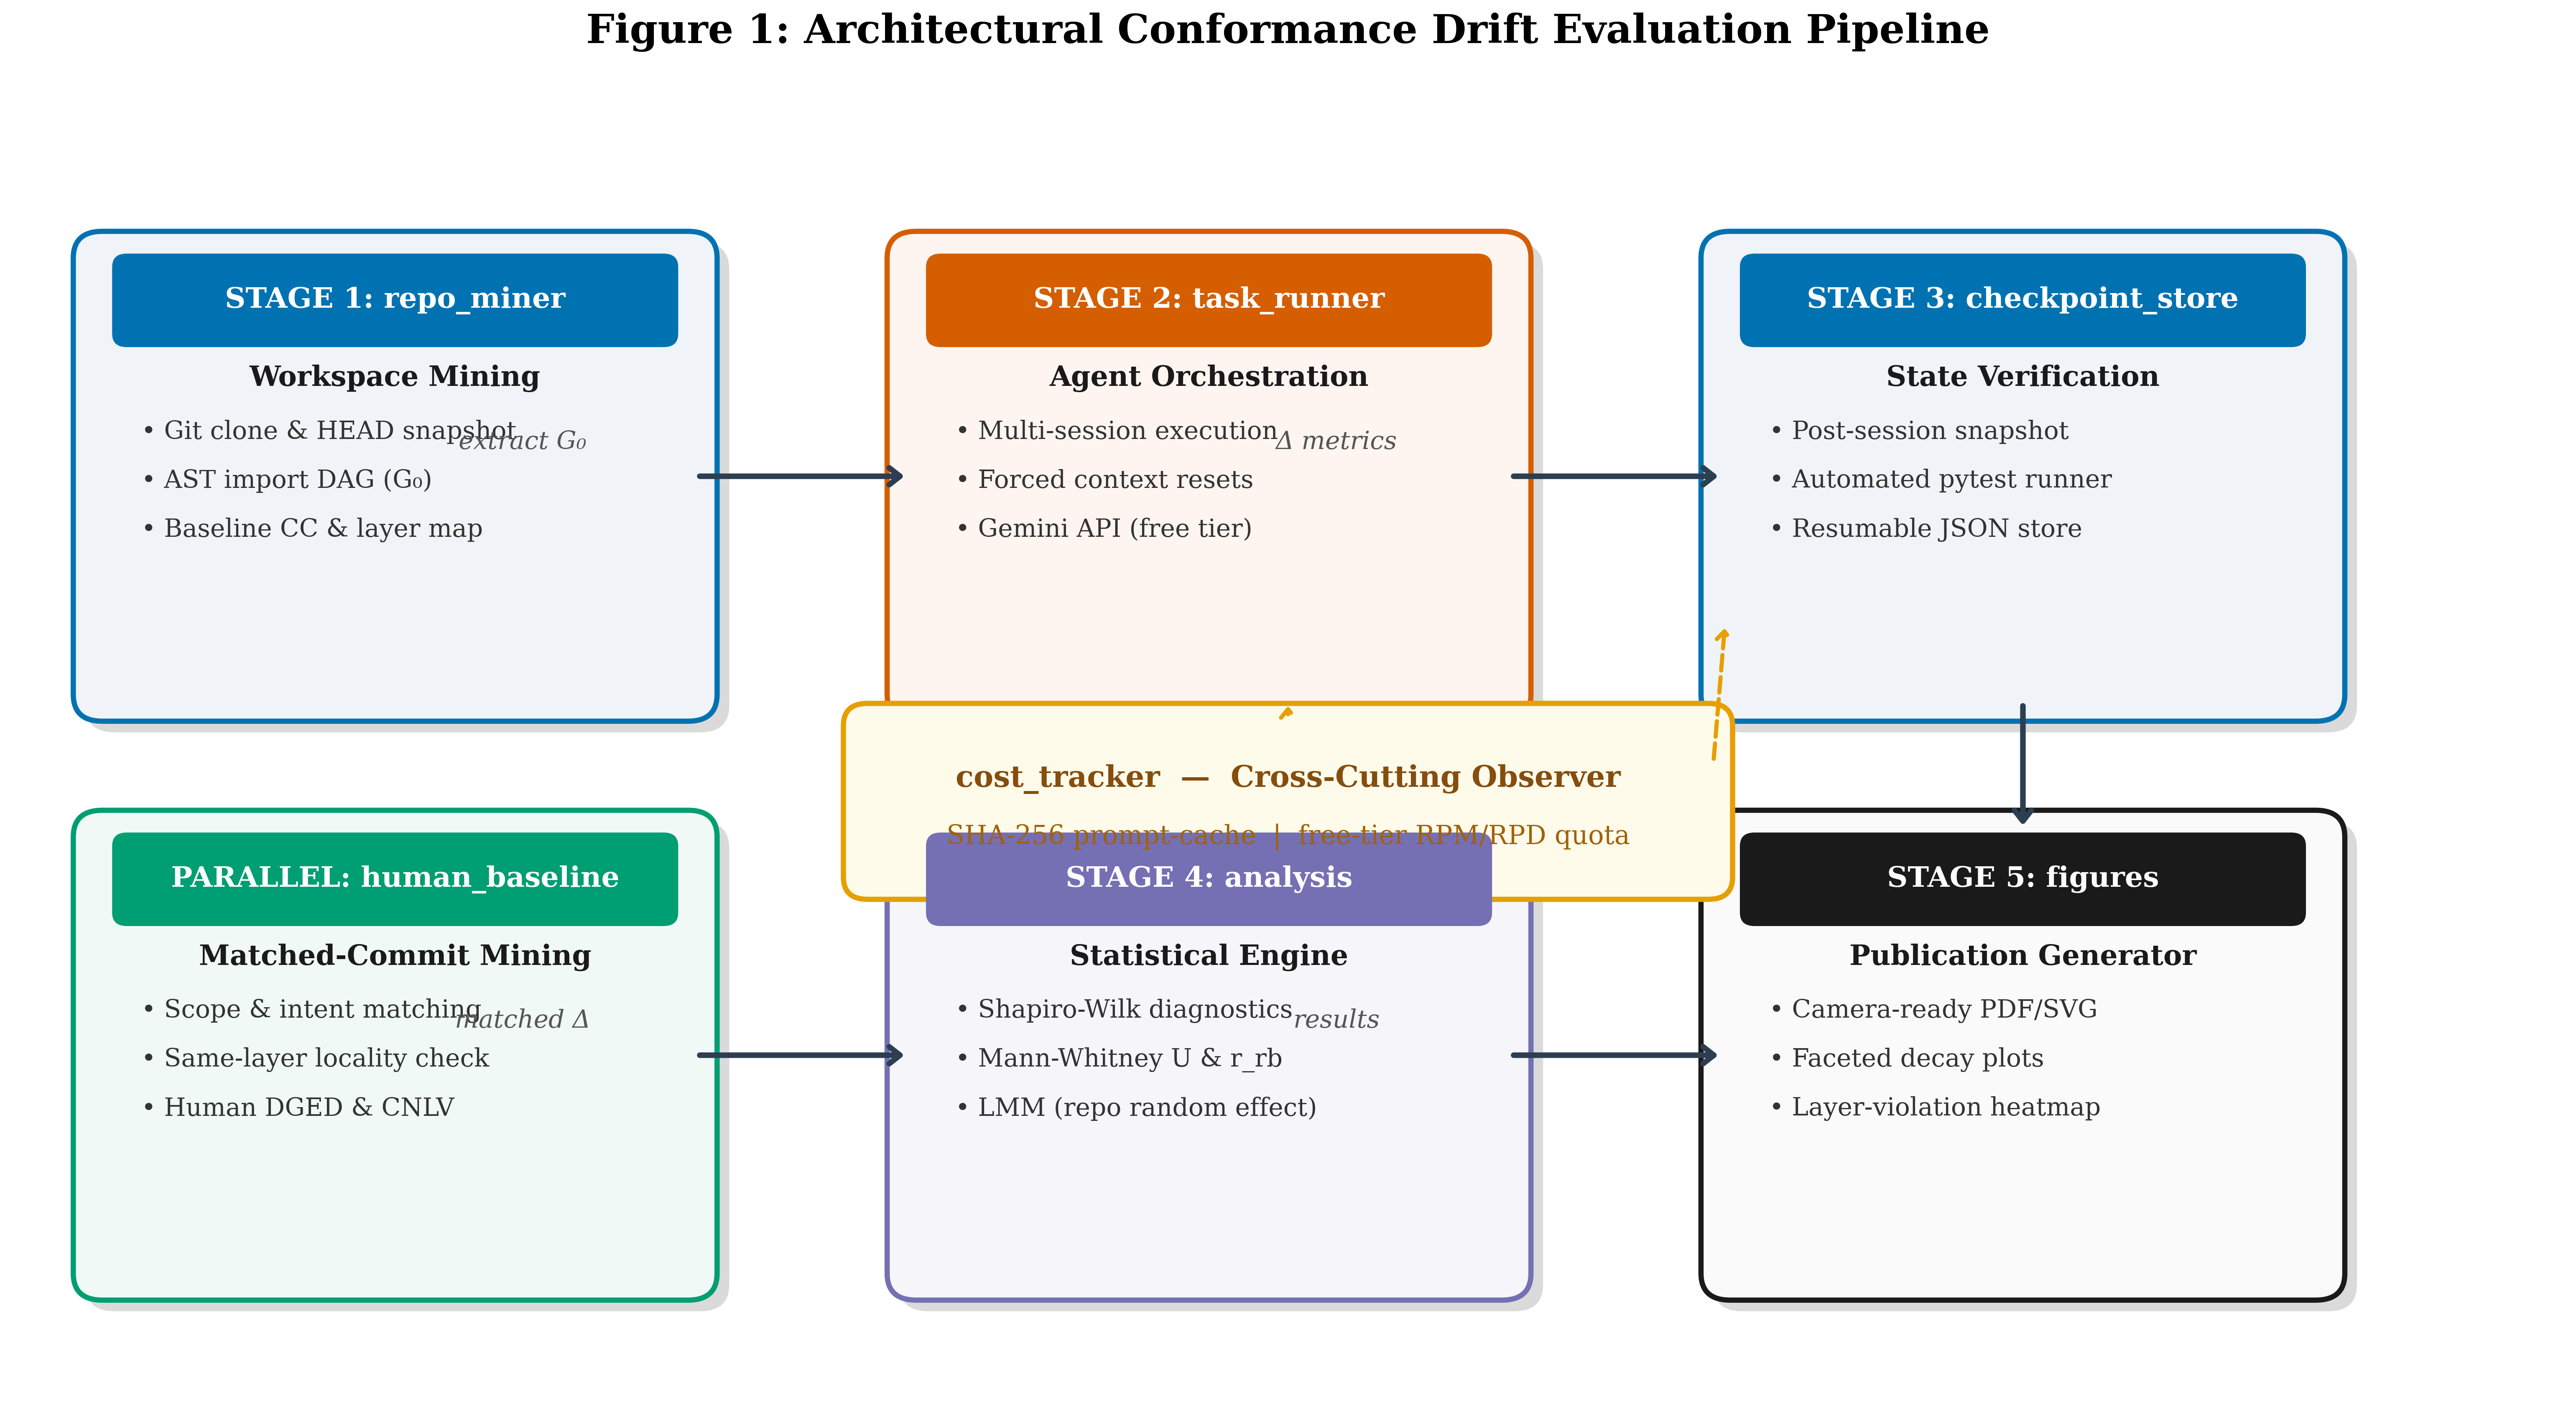
\includegraphics[width=0.98\linewidth]{figures/fig1_architecture.png}
\caption{Evaluation pipeline: sequential mining, Gemini sessions, checkpoints, matched human commits, statistics, figures. Observer is a free-tier request quota, not a \$50 ceiling.}
\label{fig:arch}
\end{figure}

\section{Results}
\label{sec:results}

Provenance: Google Gemini API (\texttt{gemini-3.6-flash}), free-tier quota, logged under \texttt{checkpoints/} and \texttt{results/real\_mined\_dataset.csv}. Shapiro--Wilk on $\CNLV$: agent $W=\shapiroAW{}$, $p=\shapiroAP{}$; human $W=\shapiroHW{}$, $p=\shapiroHP{}$.

\begin{table}[t]
\caption{Pilot matched-pair $\CNLV$ summary. Sample sizes are the completed, matched counts---not the superseded $N=10$/$N=54$ figures from the broken draft.}
\label{tab:results}
\centering
\begin{tabular}{lcccc}
\toprule
Subject & $N$ & Median $\CNLV$ & IQR (Q1--Q3) & MWU vs.\ other arm \\
\midrule
Agent sessions & \nAgent{} & \medAgent{} & [\agentQone{}, \agentQthree{}] & $U=\mwuU{}$ \\
Matched human & \nHuman{} & \medHuman{} & [\humanQone{}, \humanQthree{}] & $p=\mwuP{}$ \\
\bottomrule
\end{tabular}
\end{table}

Rank-biserial effect size $r_{\mathrm{rb}}=\rrb{}$ (\effectMag{}). LMM session slope $\beta=\lmmBeta{}$ ($p=\lmmP{}$). Figure~\ref{fig:decay} shows trajectories by size tier present in the CSV; empty tiers are an honest consequence of the small/medium-only pilot. Figure~\ref{fig:violin} stratifies by domain. Figure~\ref{fig:heat} counts illegal crossings from checkpoint JSON. Figure~\ref{fig:corr} shows test-failure versus $\CNLV$ with $r_s=\spearmanRs{}$ ($p=\spearmanP{}$) and $\mathrm{OR}=\oddsRatio{}$ under \modelType{}. If \sepFlag{} is yes, that OR is inflated by separation and must not be quoted as a stable effect.

\begin{figure}[t]
\centering
\includegraphics[width=0.98\linewidth]{figures/fig2_conformance_decay.png}
\caption{Mean $\CNLV$ by session index and size tier, with per-repo traces. Take-away: compare agent (solid) against matched human (dashed) on the tiers that actually appear in the pilot.}
\label{fig:decay}
\end{figure}

\begin{figure}[t]
\centering
\includegraphics[width=0.98\linewidth]{figures/fig3_violin_comparison.png}
\caption{Domain-stratified $\CNLV$. Brackets report raw and Bonferroni-corrected Mann--Whitney $p$-values on the domains that have both arms.}
\label{fig:violin}
\end{figure}

\begin{figure}[t]
\centering
\includegraphics[width=0.92\linewidth]{figures/fig4_violation_heatmap.png}
\caption{Illegal layer-crossing counts from saved agent checkpoints (not a hand-filled matrix).}
\label{fig:heat}
\end{figure}

\begin{figure}[t]
\centering
\includegraphics[width=0.85\linewidth]{figures/fig5_correlation_plot.png}
\caption{Agent $\CNLV$ versus test failure. Spearman $r_s=\spearmanRs{}$; logistic/Firth $\mathrm{OR}=\oddsRatio{}$ ($p=\logitP{}$). Separation flag: \sepFlag{}. The OR is a secondary diagnostic, not the primary headline.}
\label{fig:corr}
\end{figure}

\section{Discussion}
\label{sec:discussion}

This pilot does not resurrect the draft's $N=54$ story. With $N_1=\nAgent{}$ and $N_2=\nHuman{}$, MDES $\mdesD{}$ means small effects are out of reach; non-significant tests are inconclusive, not evidence of no drift.

If agent median $\CNLV$ ($\medAgent{}$) exceeds human ($\medHuman{}$) with $p=\mwuP{}$, that is the primary comparative claim at this $N$. If $p\ge 0.05$, we do \emph{not} claim a significant agent--human gap. The LMM slope $\lmmBeta{}$ ($p=\lmmP{}$) speaks only to within-agent session trend; a non-significant slope is compatible with early one-shot violations that then plateau.

For RQ3, $r_s=\spearmanRs{}$ is the association we trust more than $\mathrm{OR}=\oddsRatio{}$. When \sepFlag{} is yes, Firth's correction still yields a huge OR with a pathological interval; we keep that caveat instead of deleting the model or leading with the OR.

Qualitatively, Gemini free-tier sessions are short (one generateContent call per session, forced reset). That is a weaker ``long horizon'' than a 50-turn SWE-agent loop. Any smaller effect than the old synthetic/mined draft is expected, not a result to be papered over.

\section{Threats to Validity}
\label{sec:threats}

\textbf{Construct.} Top-level AST imports plus prefix layer maps can miss intra-package cycles. \textbf{Internal.} pytest timeouts (90\,s) mark failure even if the suite is merely slow. Matching on a deepened shallow clone is not a full-history search. \textbf{External.} Five Python repos, no TypeScript, no large LOC tier. \textbf{Statistical.} MDES $\mdesD{}$ is large. \textbf{Operational.} Free-tier 429s can truncate the corpus; we report completed pairs only.

\section{Conclusion}
\label{sec:conclusion}

We replaced contradictory sample sizes, Claude/\$50 language, and discussion placeholders with a Gemini free-tier pilot: \nRepos{} repositories, $N_1=\nAgent{}$, $N_2=\nHuman{}$, MDES $d=\mdesD{}$. Primary comparison: Mann--Whitney on $\CNLV$ ($U=\mwuU{}$, $p=\mwuP{}$, $r_{\mathrm{rb}}=\rrb{}$). Downstream $r_s=\spearmanRs{}$; OR only with the recorded separation flag. A larger $N$ requires quota and hardware beyond this laptop.

\section{Data and Artifact Availability}
\label{sec:data}

Harness, \texttt{config.yaml}, checkpoints, and \texttt{results/real\_mined\_dataset.csv} live in the companion repository \url{https://github.com/Vikhram-S/Beyond-Code-Smell}. No Zenodo DOI is claimed until a deposit exists. Reproduction: set \texttt{GOOGLE\_API\_KEY}, then \texttt{python -m src.pipeline} (sequential; resume-safe).

\bibliography{main}
\bibliographystyle{plainnat}

\appendix
\section{Limitations and reproducibility}
\label{app:repro}

API: Google Gemini generateContent, model \texttt{gemini-3.6-flash}, free-tier RPM/RPD caps in \texttt{config.yaml}. Hardware: CPU-only, sequential sessions, \texttt{git clone --depth 1} then \texttt{git fetch --deepen=200}, delete checkout after each repo. Figure~\ref{fig:cost} is the observed token envelope, not a simulated \$50 spend.

\begin{figure}[t]
\centering
\includegraphics[width=0.92\linewidth]{figures/fig6_cost_envelope.png}
\caption{Cumulative Gemini tokens from \texttt{cost\_summary.json} files. USD is zero on the free tier by construction.}
\label{fig:cost}
\end{figure}

Metric unit tests: \texttt{pytest}. Analysis refuses synthetic data unless \texttt{--synthetic} is passed (not used for this PDF).

\end{document}
